\part{Adoção de Métodos Ágeis na Gestão de Demandas de Desenvolvimento de Software}

\chapter[Adoção de Métodos Ágeis na Gestão de Demandas de Desenvolvimento de Software]{Adoção de Métodos Ágeis na Gestão de Demandas de Desenvolvimento de Software}

\section[Metodologias Ágeis de Desenvolvimento de Software]{Metodologias Ágeis de Desenvolvimento de Software}

Durante a evolução dos processos de Engenharia de Software, a indústria se baseou nos métodos tradicionais de desenvolvimento de software, que definiram por muitos anos os padrões para criação de software nos meios acadêmico e empresarial. Porém, percebendo que a indústria apresentava um grande número de casos de fracasso, alguns líderes experientes adotaram modos de trabalho que se opunham aos principais conceitos das metodologias tradicionais. Aos poucos, foram percebendo que suas formas de trabalho, apesar de não seguirem os padrões no mercado, eram bastante eficientes   \cite{filho}. 

Em 2001, 17 líderes que estavam desenvolvendo projetos de formas diferentes aos padrões até então pregados pela indústria se reuniram em uma estação de ski em Utah para discutir seus trabalhos e experiências, no final da reunião, eles formaram um grupo intitulado de Aliança de Desenvolvimento Ágil e escreveram O Manifesto Ágil, o qual é constituído de princípios e valores que o grupo considerou determinantes para bons resultados no desenvolvido de software. Com isso, os métodos de desenvolvimento de software ágeis, em contraste com os métodos tradicionais dirigidos a planos, são baseados em quatro valores advindos do Manifesto Ágil, são eles:
\begin{itemize}
\item Indivíduos e interações acima de processos e ferramentas;
\item Software operante acima de documentações grandes e completas;
\item Colaboração do cliente acima de negociações contratuais;
\item Responder à mudanças acima de seguir um planejamento.
\end{itemize}

As declarações destes valores têm um formato fácil de se identificar, a primeira parte da sentença indica a preferência, enquanto a segunda parte da sentença indica algo que, embora importante, tem prioridade menor. Assim, a Aliança e o Manifesto Ágil reconhecem a importância da documentação, processos e ferramentas, no entanto, reconhece também que a interação entre indivíduos capacitados tem ainda maior importância.

Uma documentação completa e de fácil entendimento não é ruim, porém, o foco primário deve estar no produto e na entrega de um software operante. As negociações contratuais é um prática insuficiente, os contratos podem apresentar condições de fronteiras nas quais os envolvidos podem trabalhar, mas somente com a contínua colaboração entre cliente e equipe é que se consegue entender e entregar o que o cliente realmente deseja. Assim como um plano detalhadamente elaborado do início ao fim pode ser perigoso se ele impedir que mudanças ocorram.

Os valores ágeis estão relacionados a doze princípios também advindos do Manifesto Ágil, são eles:
\begin{itemize}
\item Satisfaça o cliente por meio da entrega rápida e contínua de software que traga valor;
\item Mudanças nos requisitos são aceitas, mesmo em estágios avançados de desenvolvimento;
\item Software funcionando é entregue frequentemente em curtos períodos de tempo;
\item As pessoas relacionadas ao negócio e os desenvolvedores devem trabalhar em conjunto diariamente;
\item Construa projetos formados por indivíduos motivados, forneça o ambiente e suporte necessário e confie que eles realizarão o trabalho;
\item O modo mais eficiente e eficaz de transmitir informacoes dentro e foro do time de desenvolvimento é a comunicação face a face;
\item A principal medida de progresso é o software funcionando;
\item Processos ágeis promovem o desenvolvimento em ritmo sustentável, onde os envolvidos devem ser capazes de manter o ritmo constante;
\item Cuidar continuamente da excelência técnica e do bom design ajuda a aprimorar a agilidade;
\item Simplicidade – a arte de maximizar a quantidade de trabalho não necessário – é essencial;
\item Os melhores requisitos, arquiteturas e design surgem de equipes auto gerenciadas;
\item Em intervalos regulares, o time reflete sobre como se tornar mais eficiente, refinando e ajustando seu comportamento apropriadamente.
\end{itemize}

A partir de então diversos métodos que já eram aplicados a alguns projetos se transformaram em metodologias de desenvolvimento de software baseadas nos princípios e valores ágeis, como exemplo o Scrum e o Extreme Programming (XP). A abordagem ágil implementa os conceitos básicos de Lean no desenvolvimento de software e dá ênfase a satisfação do cliente e ao contínua melhoria dos processos de desenvolvimento de software. Os principais princípios do Lean seguidos pelas metodologias ágeis são: a entrega rápida de software funcionando e o respeito às pessoas. Dentro de cada metodologia ágil existem práticas que podem ser relacionadas aos princípios do Lean. No entanto, Lean é uma filosofia mais abrangente, enquanto a abordagem Ágil consolidou metodologias com práticas específicas, como o Scrum. 

\subsection[Scrum]{Scrum}

O Scrum é uma metodologia que começou a ser desenvolvida na década de 80, ele se concentra nos aspectos gerenciais do processo de desenvolvimento de software. É uma abordagem que favorece a construir uma equipe auto organizável e integração com outras metodologias que foquem em práticas relacionadas à programação, como o XP. 

O Scrum caracteriza-se por ser um processo empírico e adaptativo propondo iterações de curta duração (as chamadas Sprints) com reuniões de acompanhamento diárias (chamadas de Daily Meeting) realizadas de pé, as quais permitem a identificação antecipada de eventuais problemas e a visibilidade do que está sendo feito por todos. A figura 11 apresenta o ciclo de vida do processo Scrum.

\begin{figure}[h]
		\centering
		\label{fig01}
			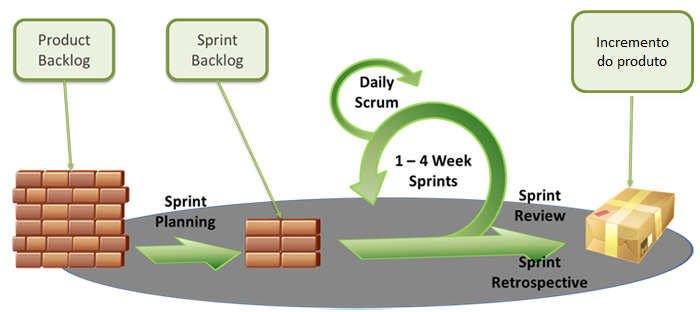
\includegraphics[scale=0.9]{figuras/scrum.png}
		\caption{Framework Scrum  \cite{scrumprocess}}
\end{figure}

No processo Scrum é definido três papéis principais: Scrum Master, aquele que deve ensinar a utilizar o Scrum, acompanhar o desenvolvimento e resolver impedimentos, Product Owner, aquele que deve garantir que o produto atenda as necessidades do cliente ou patrocinador do projeto e deve priorizar as funcionalidades que agreguem mais valor ao cliente, e Equipe de Desenvolvimento. 

No início de cada Sprint é feita uma reunião de planejamento (Sprint Planning) na qual uma estimativa e a meta da Sprint são definidas e as histórias de usuário (User Stories) que estão no Backlog do Produto são selecionadas e transformadas em tarefas do Backlog da Sprint, as quais devem ser desenvolvidas para atingir a meta da Sprint. 

Depois do planejamento, a equipe começa a fase de desenvolvimento do produto, que pode durar de uma a quatro semanas. Durante cada Sprint, o Scrum Master assegura que as histórias de usuário selecionadas não mudarão, permitindo que a equipe fique concentrada em seu objetivo. O Product Owner acompanha o desenvolvimento e esclarece eventuais dúvidas. O Product Owner só pode interferir no desenvolvimento da Sprint se uma mudança de negócio afetar os requisitos do produto que está sendo desenvolvido.

Quando uma Sprint é finalizada, a equipe de desenvolvimento apresenta o trabalho feito na reunião de revisão da Sprint (Sprint Review). O Product Owner faz testes e verifica se a meta foi realmente atingida. Ainda, após a entrega, a equipe realiza uma reunião de retrospectiva (Sprint Retrospective) para analisar seu trabalho e oportunidades de melhoria para a próxima Sprint   \cite{jeff}. 

\section[Kanban, Scrum e o Pensamento Lean ]{Kanban, Scrum e o Pensamento Lean }

Scrum e Kanban são ferramentas de processo que, em certa medida, ajuda toda a equipe a trabalhar de maneira mais eficaz, por meio de instruções do que deve ser feito. Como qualquer ferramenta, Scrum e Kanban atendem completamente a todas as situações, eles não dizem absolutamente tudo que precisa ser feito, mas sim oferecem algumas restrições e orientações. Por exemplo, o Scrum restringe um tempo fixo para cada iteração e que as equipes devem ser multifuncionais, enquanto que o Kanban restringe a utilização de quadros visíveis e a limitar o tamanho da quantidade de trabalho a ser desenvolvido em um mesmo período de tempo. A utilização de ferramentas ajuda a ter sucesso, mas não garante por si só o sucesso. Tanto Scrum quanto Kanban são empíricos no sentido que se espera que experimento o processo e o personalize as necessidades da organização.

Em termos gerais, tanto o Scrum quanto o Kanban são alinhados não só aos princípios Ágeis como também aos princípios do Pensamento Lean. Scrum e Kanban são sistemas puxados (pull), que correspondem ao princípio de gestão de inventário de Just In Time (JIT) do Lean. Isto significa que a equipe escolhe quando e quanto de trabalho irá se comprometer para então “puxar” o trabalho quando estão prontos para começar, ao invés de ter que empurrar o trabalho de algum lugar. Assim como uma impressora puxa para a próxima página somente quando está pronta para imprimi-la (embora exista um número pequeno e limitado de papel que pode ser puxado). Scrum e Kanban são baseados em otimização empírica e continua de processo, que corresponde ao princípio de Kaizen do Lean. 

Um modo de comparar estas duas ferramentas é analisando a quantidade de regras que elas oferecem. Quanto mais prescritivo é um processo mais regras estão disponíveis para seguir, não é necessário muito esforço intelectual já que as regras já estão detalhadas. Quanto mais adaptativo um processo menos regras estão definidas para serem seguidas, ou seja, pode-se fazer qualquer coisa. Evidentemente, os dois extremos desta escala não é bom   \cite{kniberg2009}. 

Os métodos ágeis são por vezes chamados de métodos “leves” por serem menos prescritivos que os métodos tradicionais devido à quantidade de atividades, papéis e artefatos definidos. Scrum e Kanban são ambos adaptativos, mas ao realizar uma comparação entre as duas ferramentas, Scrum pode ser considerado mais prescritivo que o Kanban, pois existem mais restrições, por exemplo, o Scrum prescreve o uso de iterações curtas, o Kanban não. 

\begin{figure}[h]
		\centering
		\label{fig02}
			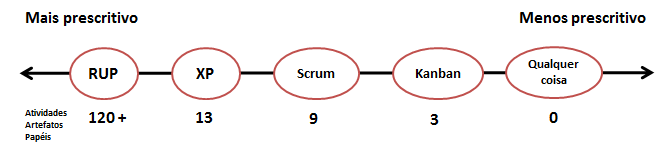
\includegraphics[scale=0.7]{figuras/prescritivo.png}
		\caption{Métodos Prescritivos}
\end{figure}

O segredo está em não se limitar ao uma única ferramenta, as ferramentas mais adaptativas podem ser combinadas de forma a trazerem mais benefícios para a organização. A maioria das equipes Scrum de sucesso incluem elementos do XP em seu processo. Muitas equipes Kanban usam as reuniões diárias advindas do Scrum. Mas é preciso ter em mente que ao retirar algo fundamental de uma metodologia, por exemplo, o tempo fixo nas iterações do Scrum, você estará utilizando algo inspirado na metodologia, uma derivação, e não mais a própria metodologia.

Com as considerações acima em mente, e considerando que ambas são excelentes para promover um fluxo contínuo e rápido de desenvolvimento de tarefas, porém é importante perceber as diferenças entre as duas ferramentas, as principais diferenças entre o Kanban e o Scrum serão apresentadas a seguir.

\subsection[Cadência]{Cadência}

O Scrum é uma única cadência de tempo fixo que combina quatro principais atividades: o planejamento, o desenvolvimento, a entrega do algo funcional e a melhoria. Uma cadência única diz respeito ao fato de manter as iterações com o mesmo tempo fixo durante um período de tempo realizando as mesmas atividades principais. Já no Kanban, não há esta prescrição de duração fixa de iterações, pode-se escolher uma periodicidade regular para realizar determinadas atividades ou pode-se escolher entregar sempre que tiver algo útil e funcional, ou seja, cadências distintas. 

\subsection[Limitação do WIP]{Limitação do WIP}

Em Scrum, o Sprint Backlog mosta quais são as tarefas a serem executadas durante a iteração atual. Geralmente, o Sprint Backlog é representado no Quadro Scrum ou Quadro de Tarefas. No Kanban, também existe o Quadro Kanban que é bastante parecido com o quadro utilizado no Scrum, em ambos há o controle das tarefas ao longo do fluxo de trabalho. As colunas de ambos os quadros podem ser determinadas a gosto. A única coisa que torna um quadro diferente do outro é que no Kanban o trabalho em progresso (WIP), na coluna “em progresso” ou nas demais colunas, é limitado explicitamente, enquanto no Scrum o limite explícito é apenas no tamanho das iterações. 

\begin{figure}[h]
		\centering
		\label{fig03}
			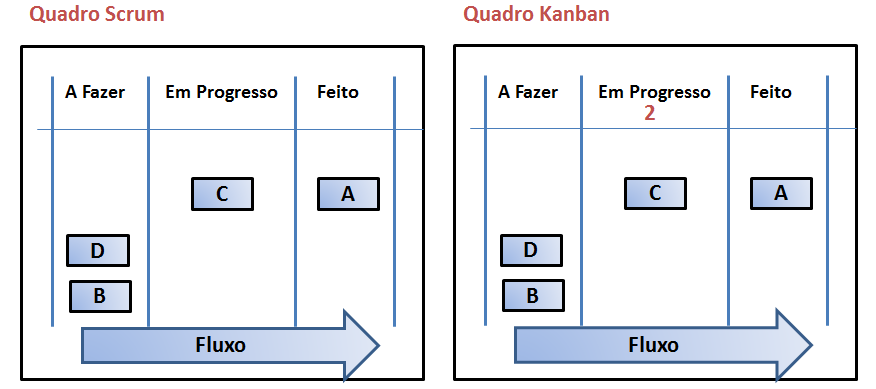
\includegraphics[scale=0.7]{figuras/quadros.png}
		\caption{Quadro Scrum x Quadro Kanban}
\end{figure}

Por vezes, uma equipe Scrum limita intuitivamente a quantidade de trabalho em progresso, evitando colocar mais atividades na coluna “em progresso” sem antes retirar as que lá estão. Quando uma equipe Scrum decide de fato limitar o WIP, então ela estará utilizando o quadro Kanban. Geralmente, as equipes Scrum medem sua velocidade (quantos pontos conseguem realizar em um determinado tempo) e com isso conseguem limitar a quantidade de trabalho em progresso.

Outra característica interessante que diferencia os dois quadros é que as tarefas no quadro do Scrum são movidas durante a iteração de forma que ao final espera-se que todas estejam na última coluna e o restante das colunas fique limpo, enquanto no quadro do Kanban sempre que uma tarefa é movida de coluna uma nova entra em seu lugar, sempre tendo tarefas em todas as colunas  \cite{kniberg2009}.

\subsection[Equipe de Trabalho]{Equipe de Trabalho}

Um quadro de Scrum pertence a exatamente uma equipe Scrum. Uma equipe Scrum é multifuncional e tem papéis definidos, ela contém todas as habilidades necessárias para completar todos os itens contidos na iteração. Um quadro de Scrum é geralmente visível a qualquer pessoa que esteja interessada, mas somente aqueles que fazem parte da equipe Scrum podem editá-lo – é a sua ferramenta para gerenciar o seu compromisso para esta iteração.

Em Kanban, equipes multifuncionais são opcionais, e o quadro de atividades não precisa pertencer exclusivamente a uma única equipe. Um quadro de atividades está relacionado a um fluxo de trabalho, não necessariamente a uma equipe.

\section[Contratação Ágil nas Organizações Públicas Brasileiras]{Contratação Ágil nas Organizações Públicas Brasileiras}

\subsection[Iniciativas de Adoção de Métodos Ágeis no Governo]{Iniciativas de Adoção de Métodos Ágeis no Governo}

As metodologias ágeis começaram a ganhar espaço no início da década de 2000 regidas pelo Manifesto Ágil e desde então vêm ganhando crescente popularidade. No cenário mundial, elas já são metodologias bastante difundidas entre diversos setores. Porém, no mercado nacional, estas metodologias são mais conhecidas e implementadas em empresas privadas. Atualmente, diversas organizações públicas brasileiras estão iniciando investimentos em adotação de contratações de fornecedores de software utilizando métodos ágeis e, portanto, estão começando a difundir tais métodos também no setor público.

Recentemente, o Tribunal de Contas da União publicou o Acórdão nº 116247 o qual contém um relatório de levantamento elaborado pela Secretaria de Fiscalização de Tecnologia da Informação (SEFTI) o qual tinha o objetivo de conhecer as bases teóricas do processo de desenvolvimento de software com metodologia ágil e conhecer experiências práticas de contratação realizadas por instituições públicas federais. As instituições analisadas foram Banco Central do Brasil (BACEN), Instituto do Patrimônio Histórico e Artístico Nacional (IPHAN), Instituto Nacinal de Estudos e Pesquisas Educacionais Anísio Texeira (INEP), Tribunal Superior do Trabalho (TST) e Supremo Tribunal Federal (STF). A seguir será relatada de forma resumida a experiência de cada instituição com o uso de metodologias ágeis em contratações de fornecedores de software de acordo com o que foi apresentado no Acórdão  \cite{TCU:2013}.

O TST publicou seu primeiro edital para contratação de horas de serviço técnico para desenvolvimento e sustentação de sistemas em 2012, antes disso o órgão adquiriu uma experiência interna de desenvolvimento de software utilizando o Scrum. As principais características do edital publicado pelo TST são: cada sprint pode agrupar manutenções de sistemas diferentes e a equipe provavelmente terá que interagir com mais de um Product Owner, pois este papel poderá ser representado por mais de uma pessoa. De acordo com o Acórdão, não foi possível analisar a gestão contratual deste órgão, pois no momento da visita não havia nenhuma ordem de serviço para este edital emitida.

O BACEN também publicou seu primeiro edital para contratação de serviço técnico de TI para desenvolvimento, documentação e manutenção de sistemas em 2012, antes disso o órgão já tinha uma experiência interna de desenvolvimento de software utilizando métodos ágeis. Os serviços de desenvolvimento e manutencao seguem o Processo dee Desenvolvimento de Software Ágil (PDS-AGIL) definido pelo BACEN baseado nas metodologias Scrum e XP, porém, por ser um processo de desenvolvimento desenhado para o uso interno, ele não deixa muito claro quais seriam as atividades de específicas para a contratação. 

O IPHAN teve sua primeira experiência com métodos ágeis no seu edital que foi publicado em 2011. Os serviços de contratação devem ser executados de acordo com a Metodologia IPHAN de Gestão de Demandas de Desenvolvimento Ágil de Software (MIDAS) definida pelo órgão. A forma de execução dos serviços prevê o desenvolvimento do projeto em ciclos e cerimônias bem definidas baseado no Scrum. Esta instituição foi escolhida para estudo de caso deste trabalho e mais detalhes sobre a metodologia de gestão de demanda utilzada serão apresentados na próxima seção. 

O INEP teve seu primeiro edtal com métodos ágeis de contratação de fábrica de sofware para prestação de serviços técnicos de TI em 2011, o qual deveria ser executado segundo a orientação da Metodologia de Desenvolvimento de Sistemas (MGDS) definida pelo INEP, que é baseada em XP e Scrum. O órgão já está no seu segundo contrato utilizando métodos ágeis. A primeira contratação fracassou porque a equipe era composta basicamente de analistas juniores e eles não tinham conhecimento em desenvolvimento de sistemas utilizando métodos ágeis. Com isso, houve uma troca de empresas e a segunda contratação, após o período de adaptação, atendeu o esperado.

O STF inicialmente implantou o desenvolvimento de sistemas utilizando metodologia ágil, baseada no Scrum, em suas equipes internas. O seu primeiro edital para contratação de empresa para prestação de serviços de desenvolvimento ágil de soluções de software foi publicado em 2012. A forma de execução dos serviços também é baseada no Scrum. Mais informações sobre a contratação não foram possíveis, pois no momento da visita da equipe de fiscalização o órgão não havia iniciado ainda a execução do contrato. 

De forma geral, o SEFTI analisou o trabalho desenvolvido nas instituições de acordo com três categorias: métrica utilizada, gestão das demandas e execução dos serviços e níveis de serviços estabelecidos. Quando a métrica utilizada, a maioria das instuições analisadas utiliza como principal métrica o Pontos de Função, com excessão do TST que utiliza a métrica Horas de Serviço Técnico. 

Quanto à forma de gestão de demandas, a maior parte do instrumento convocatório das instituições é semelhante. A demanda para construção do produto é precedida pelo planejamento do produto, o qual pode ser feito apenas pela instituição contratante ou em conjunto, entre essa e a empresa contratada. Além do planejamento do produto em si, algumas instituições também fazem o planejamento das funcionalidades que serão implementadas no próximo ciclo, iteração ou sprint, atividade preceituada no Scrum. Estas instituições emitem uma ordem de serviço por ciclo, iteração ou sprint, ou por release de software, sendo mais comum o primeiro caso. 

Quanto à aceitação do produto entregue pela contratada, embora no framework Scrum seja preceituado que ocorra na reunião de revisão da sprint, essa prática não é executada nos contratos estudados, até mesmo por impedimento normativo, como disciplinado no art. 73 da Lei 8.666/1993. Nessa ocasião, algumas instituições apenas verificam se os artefatos exigidos foram entregues, caracterizando o recebimento provisório. 

Acerca da forma de pagamento da contratada, algumas instituições remuneram os serviços de planejamento quando realizados, enquanto outras remuneram apenas os serviços de construção do software. A entrega adiantada e contínua de software, conforme postulado nos princípios dos métodos ágeis, foi observada em algumas das instituições. Para alcançar esse objetivo, elas paralelizam as atividades de preparação, execução e homologação, isto é: em um dado período de tempo, enquanto a empresa contratada executa a construção do software em um ciclo, iteração ou sprint, a contratante prepara os itens do backlog do produto. 

Quanto à execução dos serviços e níveis de serviço estabelecidos observou-se que quase todas as instituições instituíram vários níveis de serviço a serem atendidos pela contratada. Em suma, o não atendimento a critérios mínimos aceitáveis implica a redução do valor a ser pago à contratada. Dos níveis de serviço analisados, verificou-se a preocupação quase comum das contratantes com o prazo para o cumprimento das iterações, ciclos ou sprints, e com a qualidade dos produtos entregues  \cite{TCU:2013}.

\subsection[Desafios]{Desafios}

Algumas peculiaridades da Administração Pública e o seu arcabouço jurídico obrigatório (Lei 8.666/90, Instrução Normativa 04/2010 SLTI.MPOG e acórdãos do TCU) dificultam a adesão de instituições pública aos princípios Ágeis, principalmente em relação à contratação/terceirização de empresas prestadoras de serviços de desenvolvimento de software.

Ordens de Serviços, Mensuração do Produto em Pontos de Função ou Horas de Serviços Técnicos, Termo de Recebimento Provisório e Termo Definitivo, Homologações Técnicas e Negociais, Atestes e Notas Fiscais são alguns dos documentos mínimos exigidos pela legislação que o Gestor Público e a Empresa Contratada terão que produzir independentemente se a metodologia adotada é ágil ou não. Somam-se ainda todos os documentos exigidos em cláusulas contratuais   \cite{agilebrazil}. 

Como isso, o excesso de documentação poderia ser inadequado aos princípios ágeis de software funcionando mais que documentação abrangente e responder a mudanças mais que seguir um plano. Ao mesmo tempo, a falta das principais documentações exigidas pode ferir o princípio de eficiência da Administração Pública Federal (APF) e, ainda, se não seguir de forma alguma oque foi  planejado, pode-se ferir também os princípios de planejamento e economicidade da APF. 

Outro ponto relevante é a relação com equipe de desenvolvimento terceirizada. Em uma equipe externa (terceirizada), o Gestor Público não pode, por lei, interferir na conduta das pessoas contratadas, exceto via  o Preposto, pois poderia ferir o princípio de impessoalidade da APF.

Na busca pela compatibilização entre o uso de métodos ágeis e adequação a legislação pertinente, algumas alternativas tem sido adotadas por instituições públicas  em suas iniciativas recentes no uso de métodos ágeis, são elas: entrega de artefatos de documentação associados ao software produzido a cada iteração, relação contratual prevalece sobre a possível colaboração entre as partes, escopo fixo dentro das iterações e níveis de serviços vinculados à qualidade do produto   \cite{ruas}. 

Com essas alternativas, alguns dos riscos inerentes são mitigados, não há o afastamento dos princípios e da legislação aplicável e ao mesmo tempo estão encaminhadas na direção dos valores e princípios ágeis. Assim, para superar os riscos e desafios vindos do uso de métodos ágeis em contratações é preciso ser criativos, cumprir e interpretar de forma adequada as leis e valores ágeis. 

\subsection[Estudo de Caso]{Estudo de Caso}

Como estudo de caso deste trabalho é utilizada a metodologia de gestão de demandas de desenvolvimento de software ágil definida pelo IPHAN. A seguir explicaremos, além desta metodologia definida, o método Kanban utilizado para gerir as demandas.

Para desenvolver um modelo de contratação de fornecedores de software baseado em Scrum e Kanban, o IPHAN definiu alguns procedimentos que deveriam ser feitos com o foco na minimização dos riscos da execução contratual e na obtenção do sucesso no contrato de terceirização. O framework utilizado não é considerado o mais relevante, mas sim os valores e princípios do Manifesto Ágil, a entregar constante de valor e o atendimento à legislação vigente. 

As metodologias ágeis foram utilizadas como o meio para atingir o sucesso ou para identificar de forma rápida os riscos iminentes, o sucesso contratual é aquele contrato que atende às necessidades do órgão, com sistemas, sem comprometer o erário (tesouro público). Assim, para atingir sucesso em um contrato é preciso que pelos menos esses três procedimentos sejam realizados:
\begin{itemize}
\item Definir premissas nos artefatos desde o planejamento da contratação.
\item Alinhar diretrizes e condições com a Direção de TI.
\item Convalidar com a Alta Administração, ou seja, validar e sustentar essas diretrizes durante o contrato.
\end{itemize}

Com isso, foram definidas algumas premissas que devem orientar o planejamento e execução do contrato, são elas  \cite{parente}:
\begin{itemize}
\item O órgão não deve definir, ou exigir, o uso de Metodologia Ágil da entidade contratada. Não definia Metodologia de Desenvolvimento de Software (MDS), mas sim a forma de gerenciar as demandas (ordens de serviço) e os produtos que devem ser entregues e seus critérios de aceitação, a contratada pode trabalhar com a metodologia que ela quiser, porém, deve-se definir a forma de enviar e cobrar demandas, as reuniões e etc. Mesmo que esteja implicíto no edital que a metodologia ágil precisar ser implementada, pois é preciso exigir ainda a entrega de produto funcional a cada curto perído de tempo.
\item A recontagem de pontos por função nos moldes do roteiro do SISP com metodologia ágil que pode mudar constantemente é um risco. É preciso alterar o percentual definido para a alteração, manutenção ou refatoração de uma funcionalidade, definir corretamente o conceito de manutenção evolutiva, refatoração e alteração de requisito e evidenciar no processo o custo de uma alteração e fazer com que o gestor negocial, que pediu a alteração, assine a ordem de serviço e ateste a nota fiscal.
\item Só abra uma Ordem de Serviço (OS) por vez e por projeto. É preciso realizar um passo de cada vez. Pode-se ter até seis OS abertas com a Contratada, porém, será uma para cada projeto. Nunca comece oficialmente a próxima demanda sem receber ou finalizar a demanda anterior. Se a OS estiver errada ou por uma mudança negociall não for mais necessária, cancele-a e abra outra ordem de serviço que atenda a nova exigência do gestor contratual. É possível ainda abrir uma OS por Sprint.
\item Não gerencie atrasos ou defeitos. Nunca aceite que corrijam um produto com defeito dentro da mesma OS. No fim do prazo, ou sprint, receba o que estiver pronto, mesmo que não seja tudo que foi solicitado. E se nada foi entregue é uma ausência de entrega, não existe atraso, a Sprint é considerada perdida. O produto não entregue ou com defeito dever voltar para fila de demandas e entrará na próxima OS ou Sprint se o gestor negocial a quiser novamente. Se uma OS é cancelada ou se não foi entregue conforme o solicitado deve-se evidenciar no processo todas essas ocorrências.
\item Entenda a demanda antes de executá-la. É preciso planejar, pelos menos minimamente, como será o projeto, com quantas ordens de serviço o projeto será validado com o público ou órgão, qual o processo de negócio que será desenvolvido e como será a metodologia de trabalho ou gestão de demandas. É preciso saber o que será feito (a demanda) pelo menos na próxima OS ou Sprint.
\item Não aceite documentos sem sistemas. Não aceite entregas só de documentos, sem produto funcional.
\item Acredite na evoulução da empresa. A empresa irá se adequar ao processo aos poucos, no começo ela poderá não conseguir entregar o que foi solicitado ou produto funcional, mas ao longo do tempo ela irá adequar ao processo e evoluir. 
\end{itemize} 

Com estas premissas em mente o órgão definiu a Metodologia IPHAN de Gestão de Demandas de Desenvolvimento Ágil de Softwares (MIDAS) e um Kanban para auxiliar a Gestão de Demandas. O foco deste trabalho será no Kanban construído e como ele se relaciona ao MIDAS. Mais detalhes sobre o MIDAS pode ser obtido no Anexo B. 

O Kanban definido pelo IPHAN possui quatro colunas ou raias e está ilustrado na figura 14.

\begin{figure}[h]
		\centering
		\label{fig05}
			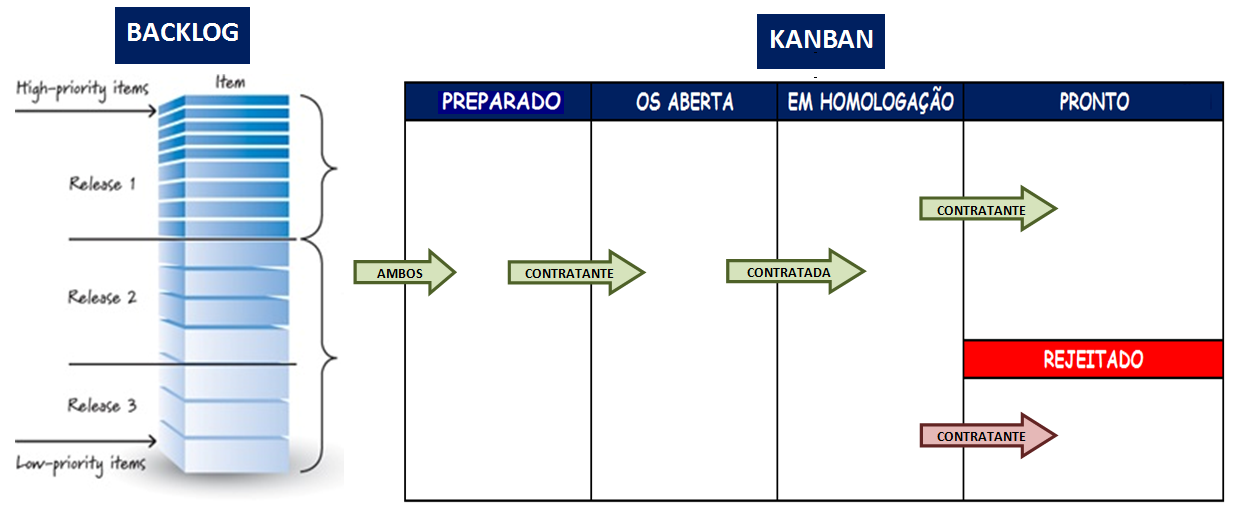
\includegraphics[scale=0.5]{figuras/kanbanIPHAN1.png}
		\caption{Quadro Kanban  \cite{parente}}
\end{figure}

A primeira raia do Kanban diz respeito aos itens que estão no estado “Preparado”. A condição de transição para esta raia pode ser feita da forma que o órgão quiser, por exemplo, os itens com mais prioridade podem ser os primeiros a irem para esta coluna. É importante que a definição de “Preparado” e a definição de “Pronto” estejam bem claras para todos os envolvidos.  

\begin{figure}[h]
		\centering
		\label{fig06}
			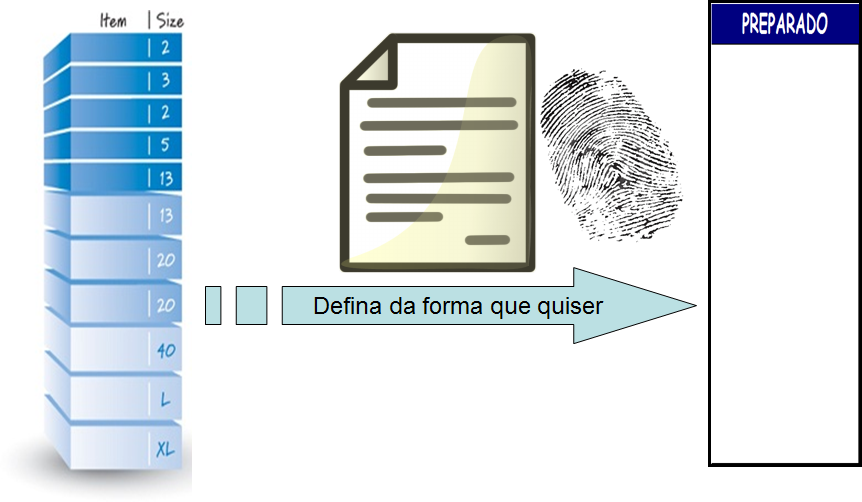
\includegraphics[scale=0.5]{figuras/kanbanIPHAN2.png}
		\caption{Transição para a raia Preparado \cite{parente}}
\end{figure}

A transição de um item da raia “Preparado” para a raia “OS Aberta” ocorre na abertura de uma ordem de serviço. Ao observamos o processo do MIDAS, vemos que essa transição ocorre após o planejamento da sprint, no subprocesso Sprint, onde uma ordem de serviço de desenvolvimento é aberta  com os itens que devem ser desenvolvidos para aquela sprint e o desenvolvimento é iniciado. 


\begin{figure}[h]
		\centering
		\label{fig07}
			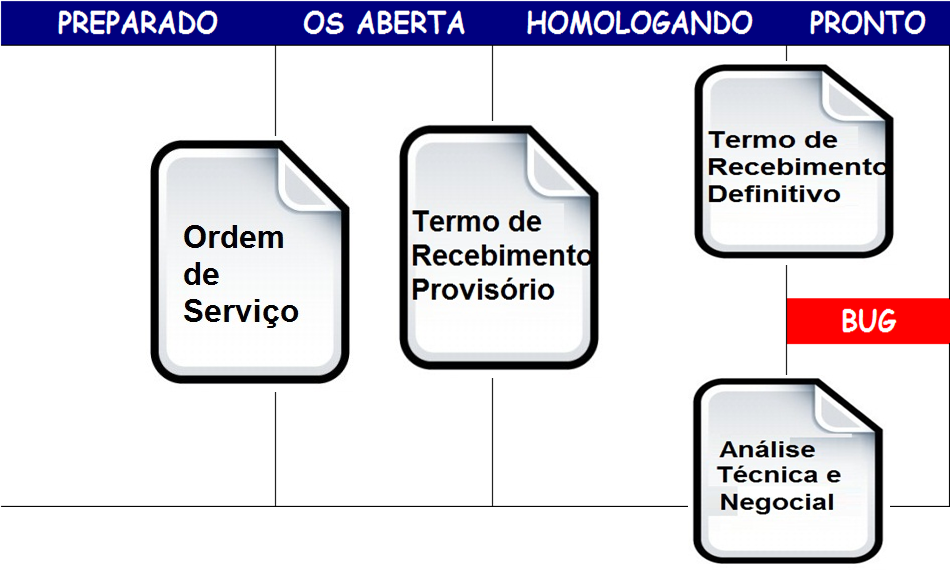
\includegraphics[scale=0.5]{figuras/kanbanIPHAN3.png}
		\caption{Transição entre raias \cite{parente}}
\end{figure}

A transição da raia “OS Aberta” para a raia “Homologando” ocorre quando o Termo de Recebimento Provisório é emitido. Ao observamos o subprocesso de Realizar Ateste Técnico no MIDAS, vemos que essa transição ocorre na atividade “Receber Produtos”, a qual tem como entrada a ordem de serviço da fase e como saída o termo de recebimento provisório. Tal atividade tem como objetivo receber os produtos definidos para a fase para posterior análise de sua aderência aos padrões e requisitos definidos. Com a emissão do termo de recebimento provisório, os produtos recebidos entram na processo de homologação. 

E a transição da raia “Homologando” para a raia “Pronto” ocorre quando o Termo de Recebimento Definitivo é emitido, ou seja, quando todos os produtos que foram anteriormente entregues são verificados e aprovados quanto a aderência aos padrões e aos requisitos a partir de uma análise técnica e negocial. Se forem detectados bugs nos produtos entregues ou se eles forem rejeitados ou tiverem necessidade de refatoração, os produtos retornam para a fila de demandas, iniciando novamente o ciclo. 


Vale ressaltar que é importante que o trabalho em progresso (WIP) seja limitado conforme o que é conceituado no método Kanban. Se as funcionalidades estão medidas por meio da técnica pontos por função, estabeleça um limite de pontos por função que podem estar em progresso em cada raia. O IPHAN definiu um limite de 200 pontos por função por raia. 

\begin{figure}[h]
		\centering
		\label{fig08}
			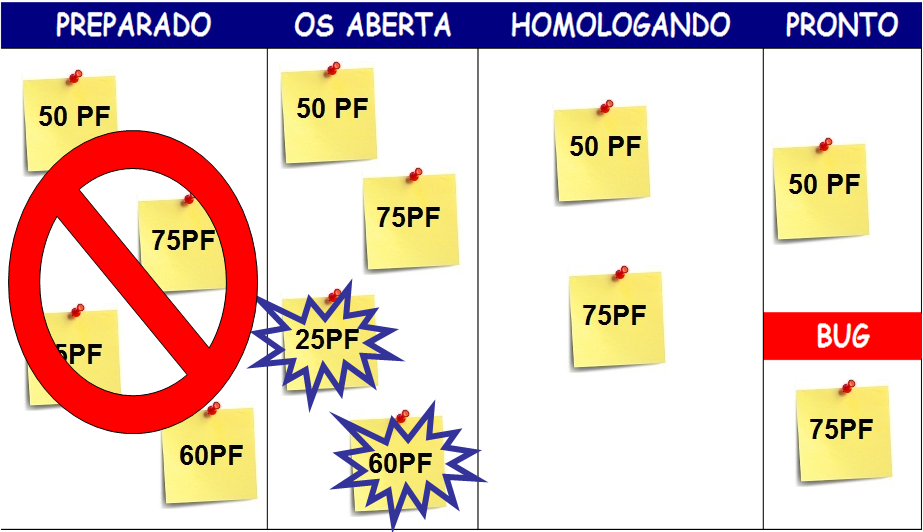
\includegraphics[scale=0.5]{figuras/kanbanIPHAN4.png}
		\caption{Limitação de WIP \cite{parente}}
\end{figure}


É importante sempre valorizar a entrega de produto funcional e não pagar por apenas documentação. Assim, divida a forma de pagamento para a Contratada em percentuais de acordo com a fase, valorizando a fase de execução como ilustrado na tabela 2.


\begin{table}[htb]
\center
\footnotesize
\begin{tabular}{|p{6cm}|p{6cm}|}
  \hline
   \textbf{Fase} & \textbf{Percentual de Pagamento}\\
    \hline
   Planejamento (1 vez) & 5\%\\
   \hline    
   Execução (n vezes) & 80\%\\
    \hline
   Encerramento (1 vez) & 15\%\\
   \hline
\end{tabular}
\caption{Formas de Pagamento}
\end{table}


Outra técnica importante é a parelização das atividades. Enquanto uma ordem de serviço está na etapa de homologação outra ordem de serviço pode ser preparada, evitando que o processo para e haja desperdício de trabalho. 

\begin{figure}[h]
		\centering
		\label{fig09}
			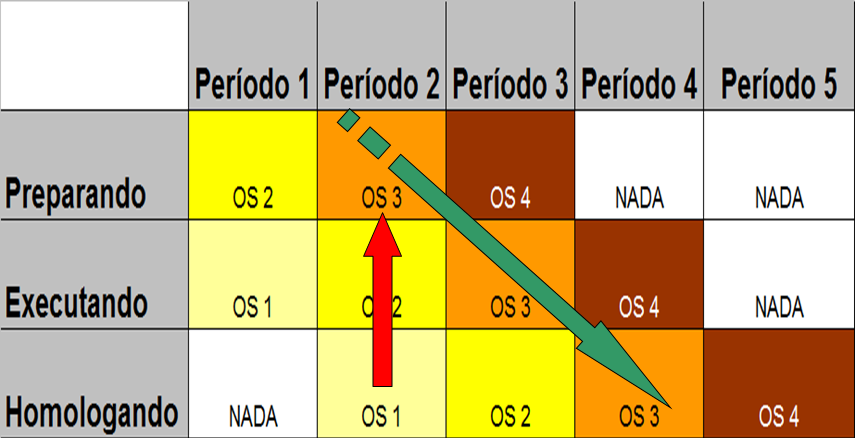
\includegraphics[scale=0.6]{figuras/kanbanIPHAN5.png}
		\caption{Parelização de Atividades \cite{parente}}
\end{figure}

O Kanban e o subprocesso de Sprint do MIDAS mostram claramente a aderência aos métodos ágeis. A paralelização das atividades, que evita desperdícios de trabalho, e a organização em fases com ciclos incrementais do MIDAS, o qual foi baseado no PDCA, mostram claramente a aderência ao Lean no desenvolvimento de software. Assim, conclui-se que as premissas utilizadas como base para o desenvolvimento do Kanban e do MIDAS foram baseadas tanto nos princípios ágeis quanto nos princípios do Lean, ressaltando a importância do envolvimento do Kanban em conjunto com os dois cenários.